\documentclass{ximera}

\newcommand{\RR}{\mathbb R}
\renewcommand{\d}{\,d}
\newcommand{\dd}[2][]{\frac{d #1}{d #2}}
\renewcommand{\l}{\ell}
\newcommand{\ddx}{\frac{d}{dx}}
\newcommand{\dfn}{\textbf}
\newcommand{\eval}[1]{\bigg[ #1 \bigg]}


\author{Jim Talamo}
\license{Creative Commons 3.0 By-bC}

\outcome{}

\begin{document}
\begin{exercise}
This exercises demonstrates an efficient way to find $f^{(35)}(0)$ for the function $f(x) = \sum_{k=0}^{\infty} \frac{2k+1}{(2k+4)!}x^{2k+3}$.  

A good way to proceed is to use the relationship between the coefficients of the power series and the derivatives of the function it represents.

\[
\textrm{If } f(x) = \sum_{k=0}^{\infty} a_k(x-c)^k, \textrm{ then: } a_n = \frac{f^{(n)}(c)}{n!}
\]

Here, $c=\answer{0}$.  In order to find $f^{(35)}(0)$, we should use $n=\answer{35}$.

The coefficient in question is thus $a_{\answer{35}}$.  

\begin{exercise}
By definition $a_{35}$ is:

\begin{multipleChoice}
\choice{Always the coefficient obtained by plugging in $k=35$.}
\choice[correct]{The coefficient in front of $(x-c)^{35}$.}
\end{multipleChoice}

In this case, we find $x^{2k+3}=x^{35}$ when $k=\answer{16}$, so:

\[
a_{35} =  \frac{2k+1}{(2k+4)!} \bigg|_{k=\answer{16}} = \frac{\answer{33}}{\answer{36!}}
\]

\begin{exercise}
We now use the formula $a_n = \frac{f^{(n)}(c)}{n!}$ to find:

\begin{align*}
a_{35} &= \frac{f^{(35)}(0)}{35!} \\
\answer{\frac{33}{36!}} &= \frac{f^{(35)}(0)}{\answer{35!}}
\end{align*}

\begin{exercise}
Thus, $f{(35)}(0) = \frac{33 \cdot 35!}{36!} = \answer{\frac{11}{12}}$.

(use properties of factorials to type a simplified answer)

\begin{exercise}
There is another way to proceed here that is less notationally
friendly, but it is instructive to point it out since it highlights
the logic behind the formula we used.  Note that we can write out the
series represented by :

$f(x) = \sum_{k=0}^{\infty} \frac{2k+1}{(2k+4)!}x^{2k+3}:$

\begin{image}
  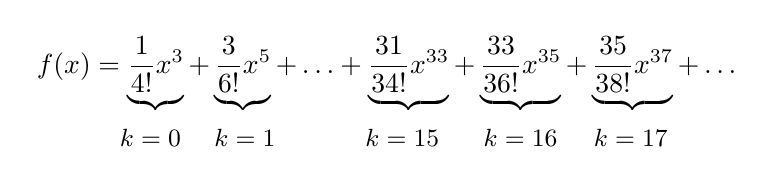
\begin{tikzpicture}
        \node at (0,0) {
          $f(x)= \underbrace{\frac{1}{4!}x^3}+\underbrace{\frac{3}{6!}x^5}+\ldots+\underbrace{\frac{31}{34!}x^{33}}+ \underbrace{\frac{33}{36!}x^{35}} + \underbrace{\frac{35}{38!}x^{37}}+\ldots$};
        \node at (-3,-.8) {\small{$k=0$}}; 
        \node at (-1.8,-.8) {\small{$k=1$}}; 
        \node at (.2,-.8) {\small{$k=15$}}; 
        \node at (1.7,-.8) {\small{$k=16$}};
        \node at (3.1,-.8) {\small{$k=17$}};  
             \end{tikzpicture}
  \end{image}

Now, as we've seen previously, if we compute $35$ derivatives:

\begin{image}
  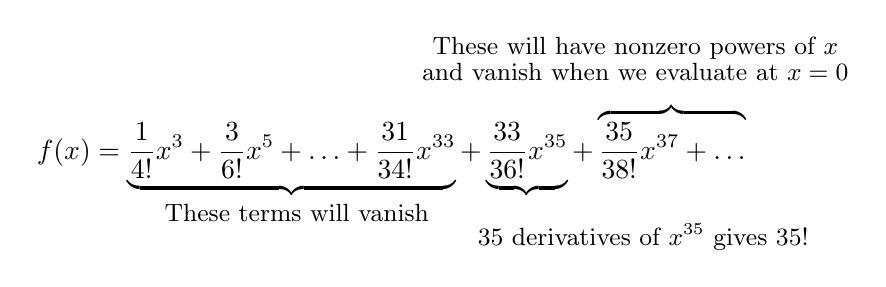
\begin{tikzpicture}
        \node at (0,0) {
          $f(x)= \underbrace{\frac{1}{4!}x^3+\frac{3}{6!}x^5+\ldots+\frac{31}{34!}x^{33}}+ \underbrace{\frac{33}{36!}x^{35}} + \overbrace{\frac{35}{38!}x^{37}+\ldots}$};
        \node at (-1.2,-.8) {\small{These terms will vanish}}; 
        \node at (3.2,-1.1) {\small{$35$ derivatives of $x^{35}$ gives $35!$}};
        \node at (3.1,1.3) {\small{These will have nonzero powers of $x$}};  
        \node at (3.1,1) {\small{and vanish when we evaluate at $x=0$}};  
             \end{tikzpicture}
  \end{image}
  
Thus, $f^{(35)}(0) = \frac{33}{36!} \cdot \answer{35}!$ via these observations.  

Does this match the result from before?

\begin{multipleChoice}
\choice[correct]{Yes}
\choice{No}
\end{multipleChoice}  
 
 This hopefully is not surprising; it is precisely these observations that led to the formula $a_n = \frac{f^{(n)}(c)}{n!}$ in the first place!  

\end{exercise}
\end{exercise}
\end{exercise}
\end{exercise}



\end{exercise}
\end{document}
